\documentclass[10pt]{beamer}

\usepackage[T1]{fontenc}
\usepackage{lmodern}
\usepackage{amsmath,amssymb}
\usepackage{booktabs}
\usepackage{graphicx}

\usepackage{xjtu}
\setbeamertemplate{background}{%
  
\includegraphics[width=\paperwidth,height=\paperheight]{assets/xjtu_background.png}}
\setbeamertemplate{navigation symbols}{}
\setbeamersize{text margin left=0.55cm,text margin right=0.55cm}

\title{Programmatic Modeling of Concurrent Composition\\and High-Order Observers}
\subtitle{Labeled Finite-State Automata}
\author{Zixi Wang}
\institute{Xi'an Jiaotong University}
\date{Summer Research Presentation}

\begin{document}

\begin{frame}
  \titlepage
  \begin{center}
    \vspace{-0.45cm}
    
\includegraphics[width=0.14\linewidth]{assets/xjtu_logo.png}
  \end{center}
\end{frame}

\begin{frame}{Problem Setting}
  Consider a finite-state system $G$ observed by two agents.

  \vspace{0.3cm}
  \begin{itemize}
    \item Agent $A_1$ estimates the current state of $G$ from its observations.
    \item Agent $A_2$ has a different observation of the same execution.
    \item Agent $A_2$ infers the possible state estimates held by Agent $A_1$.
  \end{itemize}

  \vspace{0.35cm}
  \begin{block}{Target computation}
    For an observation $\beta$ of Agent $A_2$, compute
    \[
      M_{A_1\leftarrow A_2}(G,\beta)
      =\{M_1(G,\ell_1(s)):s\in L(G),\ \ell_2(s)=\beta\}.
    \]
  \end{block}
\end{frame}

\begin{frame}{LFSA Observer and Concurrent Composition}
  \small
  \textbf{Labeled finite-state automaton}
  \[
    S=(Q,E,\delta,Q_0,\Sigma,\ell),
    \qquad \ell:E\rightarrow\Sigma\cup\{\epsilon\}.
  \]
  The labeling function models what an agent observes.

  \vspace{0.18cm}
  \textbf{Observer}
  \[
    \delta_{\mathrm{obs}}(q_{0,\mathrm{obs}},\alpha)=M(S,\alpha)\subseteq Q.
  \]
  Each observer state is one current-state estimate.

  \vspace{0.18cm}
  \textbf{Concurrent composition}
  \[
    CC(S_1,S_2)
  \]
  It synchronizes transitions with equal observable labels and interleaves
  unobservable transitions.
  \vfill
  {\tiny Source: Zhang, \textit{Annual Reviews in Control}, 56, 100902, 2023.}
\end{frame}

\begin{frame}{Order-2 Observer Pipeline}
  \small
  \begin{tabular}{@{}cll@{}}
    \toprule
    \textbf{Stage} & \textbf{Transformation} & \textbf{Program} \\
    \midrule
    1 & Add Agent $A_1$ labels to $G$ & \texttt{fa\_agent\_to\_lfsa.py} \\
    2 & Build $A_1$'s observer & \texttt{observer.py} \\
    3 & Compose the system and observer & \texttt{CC.py} \\
    4 & Recover the underlying event system & \texttt{lfsa\_to\_fa.py} \\
    5 & Replace labels with Agent $A_2$'s view & \texttt{fa\_agent\_to\_lfsa.py} \\
    6 & Build $A_2$'s observer & \texttt{observer.py} \\
    \bottomrule
  \end{tabular}
  \vspace{0.45cm}
  \begin{block}{Programmatic data flow}
    \[
      (G,A_1,A_2)\longrightarrow Obs_{A_1}
      \longrightarrow CC\longrightarrow Obs_{A_1\leftarrow A_2}(G).
    \]
  \end{block}
\end{frame}

\begin{frame}{Theorem 25 and Example 27}
  \begin{columns}[T,onlytextwidth]
    \begin{column}{0.47\textwidth}
      \small
      If reading $\beta$ reaches the order-2 observer state
      \[
        \{(q_1,X_1),\ldots,(q_n,X_n)\},
      \]
      then Theorem 25 gives
      \[
        M_{A_1\leftarrow A_2}(G,\beta)
        =\{X_1,\ldots,X_n\}.
      \]
      The second components are precisely the possible estimates of Agent $A_1$.
    \end{column}
    \begin{column}{0.50\textwidth}
      \centering
      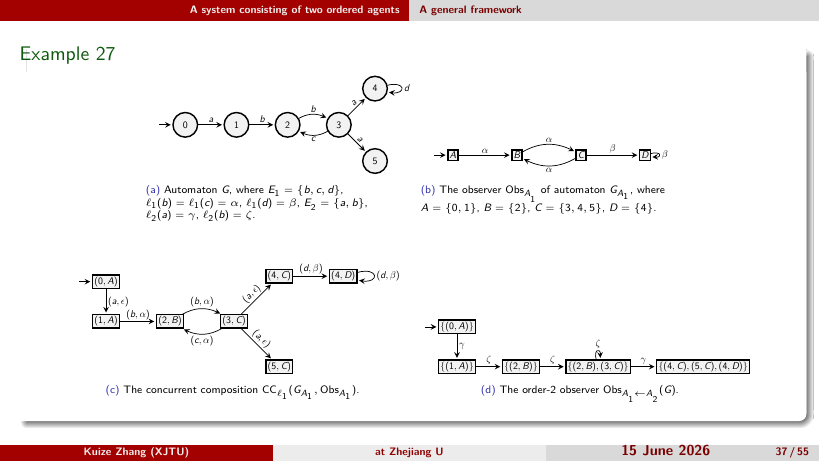
\includegraphics[width=\linewidth,trim=20 12 20 42,clip]{assets/example27_reference.png}
      \vspace{0.12cm}

      \scriptsize
      The implementation reproduces the published five-state,
      five-transition order-2 observer.
    \end{column}
  \end{columns}
  \vfill
  {\tiny Reference figure: Zhang et al., \textit{High-Order Observers and High-Order State-Estimation-Based Properties}, Example 27.}
\end{frame}

\begin{frame}{Complexity and Summary}
  Let $n=|Q|$. In the worst case,
  \[
    |Obs_{A_1}|\leq 2^n,
    \qquad
    |CC|\leq n2^n,
    \qquad
    |Obs_{A_1\leftarrow A_2}|\leq 2^{n2^n}.
  \]
  Therefore, explicit construction has a double-exponential upper bound
  in both time and storage, although only reachable states are generated.

  \vspace{0.35cm}
  \textbf{Summary}
  \begin{itemize}
    \item The programs implement LFSA conversion, observers, and concurrent composition.
    \item The resulting order-2 observer computes Agent $A_2$'s possible inferences about Agent $A_1$.
    \item Example 27 provides an end-to-end validation case.
  \end{itemize}
\end{frame}

\end{document}
